%% Copernicus Publications Manuscript Preparation Template for LaTeX Submissions
%% ---------------------------------
%% This template should be used for the following class files: copernicus.cls, copernicus2.cls, copernicus_discussions.cls
%% The class files, the Copernicus LaTeX Manual with detailed explanations regarding the comments
%% and some style files are bundled in the Copernicus Latex Package which can be downloaded from the different journal webpages.
%% For further assistance please contact the Publication Production Office (production@copernicus.org).
%% http://publications.copernicus.org


%% Differing comments regarding the specific class files are highlighted.


%% copernicus.cls
\documentclass[acp]{copernicus}

%% copernicus2.cls
%\documentclass[acp]{copernicus2}

%% copernicus_discussions.cls
%\documentclass[journal abbreviation, hvmath, online]{copernicus_discussions}


\begin{document}


\title{Something about cloud tracking}


\author[1]{Jordan T Dawe}
\author[1]{Philip H Austin}

\affil[1]{Department of Earth and Ocean Sciences, 
        University of British Columbia, 
	6339 Stores Road, 
        Vancouver, BC, 
        V6T 1Z4}

%% The [] brackets identify the author to the corresponding affiliation, 1, 2, 3, etc. should be inserted.



\runningtitle{CLOUD TRACKING}

\runningauthor{Dawe and Austin}

\correspondence{Jordan T Dawe\\ (jdawe@eos.ubc.ca)}



\received{}
\pubdiscuss{} %% only important for two-stage journals
\revised{}
\accepted{}
\published{}

%% These dates will be inserted by the Publication Production Office during the typesetting process.


\firstpage{1}

\maketitle



\begin{abstract}
A technique for the tracking of individual clouds in an large eddy 
simulation model is presented.  We use this technique on a LES of a 
shallow cumulus cloud field based upon the Barbados Oceanographic and 
Meteorological Experiment (BOMEX), to calculate statistics of cloud 
height, lifetime, and other physical properies for individual clouds 
in the model.  We also examine the question of nature versus nurture 
in cloud fields: do cloud-base properties determine the properties 
of the clouds (nature), or are cloud properties determined by the 
environmental conditions they encounter (nurture).  We find that clouds 
which ascend through an environment that has been pre-moistened by 
previous cloud activity are no more likely to reach the inversion than 
clouds that ascend through a drier environment.  Conversely, we find 
that cloud base moisture and liquid-water potential temperature are 
largely uncorrelated with cloud properties, but that the area of the 
cloud base exerts strong controls over cloud buoyancy, vertical velocity, 
and maximum cloud height.
\end{abstract}


%% only used for copernicus2.cls
%\abstract{
% TEXT
% \keywords{TEXT}}



\introduction
%% \introduction[modified heading if necessary]

Clouds are vital for climate
hard to parameterize
Studied via LES
LES studies traditionally look at bulk cloud properties

Individual plumes
Arakawa and Shubert
Zhao and Austin (
Heus and Jonkers

Satellite cloud tracking/cloud identification.

Better would be an automated system




Here we present a fully automated algorithm for the tracking of individual 
clouds in a LES.  In section 2 we describe the BOMEX LES we analyzed, section 3 
presents the cloud tracking algorithm itself, and section 4 presents an overview 
of the statistics generated by the algorithm.  Then in section 5 we use the 
output generated by the algorithm to address the question of whether initial 
cloud properties or the environment encountered by the cloud is more important 
in determining the course of the cloud's life cycle.  Finally in section 6 
we discuss our results and conclusions.

%==============================================================================

\section{Model Description}

All LES calculations in this paper were made using the System for Atmospheric 
Modeling \citep[SAM;][]{Khairoutdinov2003}.  SAM is an anelastic LES 

The model was run configured as standard Global Energy and Water
Cycle Experiment (GEWEX) Cloud System Studies \citep[GCSS;][]{Randall2003}
Barbados Oceanographic and Meteorological Experiment 
\citep[BOMEX;][]{Siebesma2003} experiment.  BOMEX simulates a trade-wind cumulus 
cloud field observed over ocean near Bermuda

The BOMEX run was performed on a 6.4 km x 6.4 km horizontal x 3.2 km vertical 
domain with 25 meter grid resolution in all directions for 6 hours, and the 
first three hours of simulation were discarded. 

%==============================================================================

\section{Cloud Tracking}

Dividing a cloud field up into individual clouds at a single moment in time is 
a trivial matter of finding connected cloudy regions.  Tracking the resulting 
clouds from one time step to the next is more problematic, as a cloud is not a 
consistent physical object; it is, rather, a series of processes.  A rising 
parcel of moist air may condense, a parcel of air containing condensate may 
evaporate, and a cloud may merge with another cloud or split into multiple 
clouds.  To handle all of these processes, we adopt a more complex definition 
of what constitutes an individual cloud.

We begin by defining three cloud regions.  The first is the cloud ``core", 
defined following \cite{Siebesma1995} as all model points containing condensed 
liquid water which have positive buoyancy and upward velocity.  The second we 
refer to as the ``condensed" region, defined simply as all model points 
containing condensed liquid water.  Third is the cloud ``plume", the region of 
upward moving air that is associated with the cloud.  We define this region 
following the work of \cite{Couvreaux2010} via a numerical tracer that is 
emitted at the surface and subsequently decays exponentially with a one minute 
time constant.  A point is considered to be in the plume if the tracer value of 
that point is larger than one standard deviation above the mean tracer value at 
the current height.  Additionally, the tracer must exceed five precent of the 
integral of the tracer standard deviation from the surface to the current 
height.  However, unlike Couvreaux et al., we do not require upper-level plume 
points to have condensed liquid water.  Finally, we force the condensed region 
to be a subset of the plume by setting all condensed points to also be plume 
points.

Next, we divide the cloud field into ``cloudlets" by assigning core points 
which are nearest-neighbour adjacent to the same cloudlet.  These core 
cloudlets are then expanded into nearest-neighbour connected condensed points 
until all condensed points that are connected to a core are assigned to a 
cloudlet.  Condensed points cannot belong to two cloudlets, so if a cloud 
contains more than one contiguous volume of nearest-neighbour connected core 
points it will be split into seperate cloudlets.  Leftover condensed points are 
then divided into new cloudlets which have no cores.  Once all the condensed 
points have been assigned to cloudlets, this expansion process is repeated for 
the plume points.  This results in three types of cloudlets: ones consisting of 
core points surrounded by condensed points surrounded by plume, ones consisting 
of condensed points surrounded by plume, and ones consisting only of plume 
points.  This process is then repeated for every saved model time step.

These cloudlets are then assigned to individual clouds.  For the first time 
step, we assign cloudlets which have touching condensed surfaces to the same 
cloud.  At subsequent time steps, cloudlets that spatially overlap with a cloud 
at the previous timestep are assumed to be the same cloud.  The cloudlet's 
position is corrected for advection using the mean velocity of the cloudlet's 
condensed points (if condensed points are present in the cloudlet) or plume 
(if they are not), multiplied by the time between model output saves.

Four kinds of overlap are possible: condensed points in the cloudlet may 
overlap condensed points in a previous time step cloud 
(condensed$\rightarrow$condensed); condensed points may overlap previous plume 
points (plume$\rightarrow$condensed); plume may overlap condensed points 
(condensed$\rightarrow$plume); and plume may overlap plume 
(plume$\rightarrow$plume).  Several kinds of overlap may occur simultaneously, 
so we define a heirarchy of connection types and check each in turn.  The 
strongest connection type is condensed$\rightarrow$condensed, followed by 
plume$\rightarrow$condensed, then plume$\rightarrow$plume.  
Condensed$\rightarrow$plume connections are ignored, which prevents 
connections between newly formed cloudlets and leftover plume from a 
dissipating cloud.  Conversely, allowing plume$\rightarrow$condensed 
connections lets us associate newly condensed clouds with plumes rising through 
the sub-cloud layer.  Only the strongest connection type present for a given 
cloudlet is considered: if a cloudlet has condensed$\rightarrow$condensed 
connections, any condensed$\rightarrow$plume or plume$\rightarrow$plume 
connections are ignored, and if there are condensed$\rightarrow$plume 
connections, plume$\rightarrow$plume connections are ignored.  

A cloudlet may connect to more than one cloud, which is used to identify 
merges and splits.  Any cloudlet which overlaps more than one previous time 
step cloud is considered to be the result of a merge between the two clouds.  
In this case the cloudlet is assigned to the cloud with the largest overlap, 
and the other overlapping clouds are assumed to have merged with the largest 
overlap cloud.  Next, clouds that connect to more than one cloudlet are 
considered for splitting.  Splits occur only if a cloud contains more than one 
cloudlet whose plume is in contact with the ground, with the largest cloudlet 
being assigned to the original cloud and the smaller sub-clouds becoming new 
clouds.  Cloudlets which are not connected to the ground are assigned to the 
nearest ground-connected cloudlet, measured by the distance between the 
centroids of the cloudlets.  Any cloudlets that do not overlap clouds in the 
previous time step are assumed to be new clouds.  This process of cloudlet 
assignment, merging, splitting, and creation is repeated for each time step 
until all cloudlets are assigned to a cloud.
  
Once the cloudlets are all assigned to a cloud, any cloud that has cloud core 
points for less than five minutes is flagged as noise.  If any merge or split 
events occured over these clouds' short lifetimes, the noise cloud is rejoined 
to the cloud it split from or merged into.  This prevents decaying detritus shed 
from a cloud top, or clouds which split then immediately re-merge with their 
parent, from being counted as discrete cloud objects.  Remaining noise clouds 
are separated from the main cloud database and considered to be a mixture of 
``mistakes" in the tracking algorithm and short-lived, dynamically forced clouds 
at cloud base.


%==============================================================================

\section{Tracked Cloud Statistics}

First we examine the population statistics of the tracked cloud ensembles we 
have isolated with our tracking algorithm for the BOMEX GCSS case.


%==============================================================================

\section{Nature versus Nurture}
TEXT

Bonferroni Correction!!!

\subsection{Cloudbase Properties}

\subsection{Cloud Environment}

%==============================================================================

\conclusions
%% \conclusions[modified heading if necessary]
TEXT


%\appendix
%\section{\\ \\ \hspace*{-7mm} HEADING}    %% Appendix A

%\subsection                               %% Appendix A1, A2, etc.

\begin{acknowledgements}
Support for this research was provided by the Canadian Foundation for Climate 
and Atmospheric Science through the Cloud Aerosol Feedback and Climate 
network.  Figures were generated using the matplotlib library in the Python
programming language.
\end{acknowledgements}


\bibliographystyle{copernicus}
\bibliography{./bibliography/cloud_tracking}


%% Literature citations
%% command                        & example result
%% \citet{jones90}|               & Jones et al.\ (1990)
%% \citep{jones90}|               & (Jones et al., 1990)
%% \citep{jones90,jones93}|       & (Jones et al., 1990, 1993)
%% \citep[p.~32]{jones90}|        & (Jones et al., 1990, p.~32)
%% \citep[e.g.,][]{jones90}|      & (e.g., Jones et al., 1990)
%% \citep[e.g.,][p.~32]{jones90}| & (e.g., Jones et al., 1990, p.~32)
%% \citeauthor{jones90}|          & Jones et al.
%% \citeyear{jones90}|            & 1990






%% FIGURES %%%%%%%%%%%%%%%%%%%%%%%%%%%%%%%%%%%%%%%%%%%%%%%%%%%%%%%%%%%%%%%%%%%%


%% ONE-COLUMN FIGURES

%f
%\begin{figure}[t]
%\vspace*{2mm}
%\begin{center}
%\includegraphics[width=8.3cm]{./figures/figure1}
%\end{center}
%\caption{Schematic representation of our cloudlet algorithm.}
%\label{fig:cloudfinder_instructions}
%\end{figure}


%% TWO-COLUMN FIGURES

%f
\begin{figure*}[t]
\vspace*{2mm}
\begin{center}
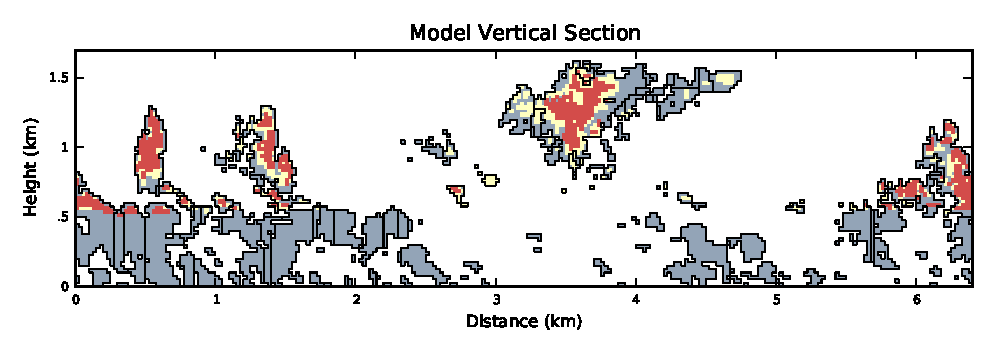
\includegraphics[width=\textwidth]{./figures/vertical_section}
\end{center}
\caption{Vertical section through the BOMEX model, showing the cloud core
(black), the cloud (dark grey) and the plume (light grey) regions used by the 
cloud tracking algorithm.}
\label{fig:cloudfinder_instructions}
\end{figure*}

%f
\begin{figure*}[t]
\vspace*{2mm}
\begin{center}
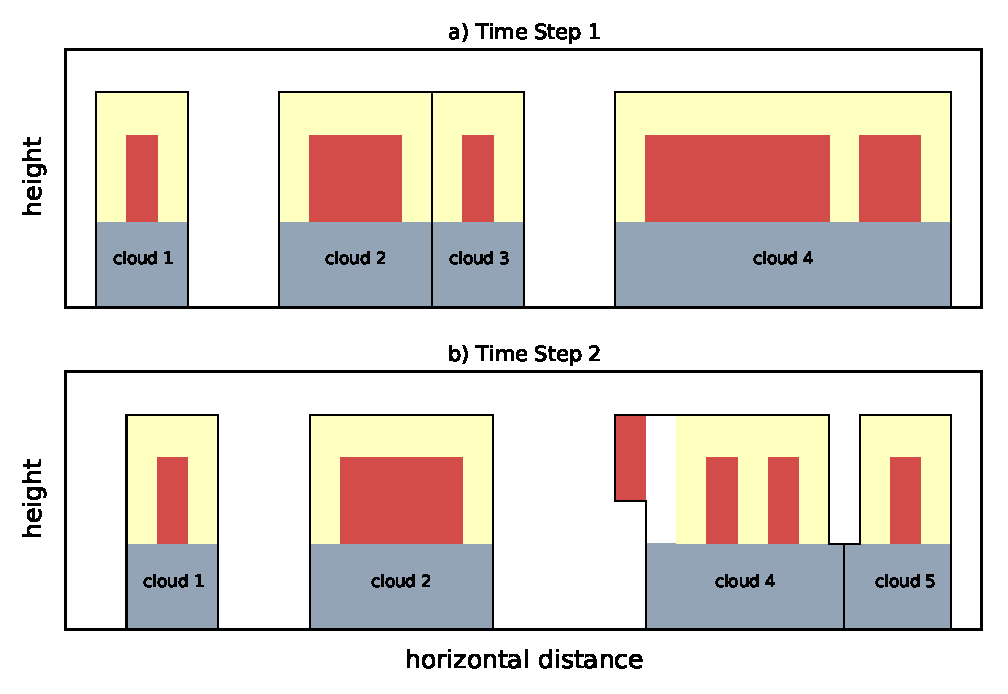
\includegraphics[width=\textwidth]{./figures/cloudfinder_instructions}
\end{center}
\caption{Schematic representation of our cloud tracking algorithm.}
\label{fig:cloudfinder_instructions}
\end{figure*}

%f
\begin{figure*}[t]
\vspace*{2mm}
\begin{center}
\includegraphics[width=\textwidth]{./figures/example_clouds}
\end{center}
\caption{Height-time profiles of the longest-lived cloud in the BOMEX 
simulation.}
\label{fig:example_clouds}
\end{figure*}

%f
\begin{figure}[t]
\vspace*{2mm}
\begin{center}
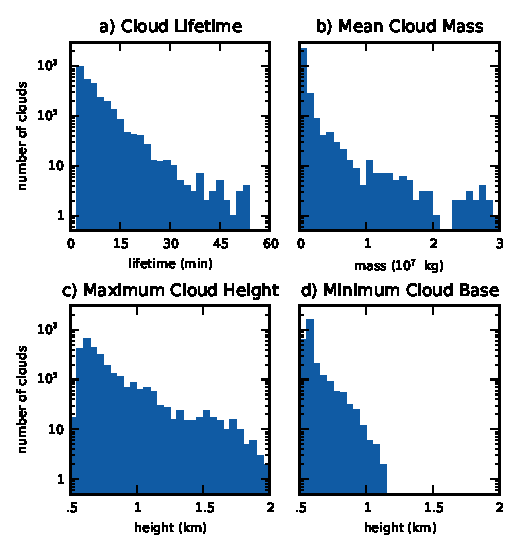
\includegraphics[width=8.3cm]{./figures/cloud_stats}
\end{center}
\caption{Histograms of cloud lifetimes and heights.}
\label{fig:cloud_stats}
\end{figure}

%f
\begin{figure*}[t]
\vspace*{2mm}
\begin{center}
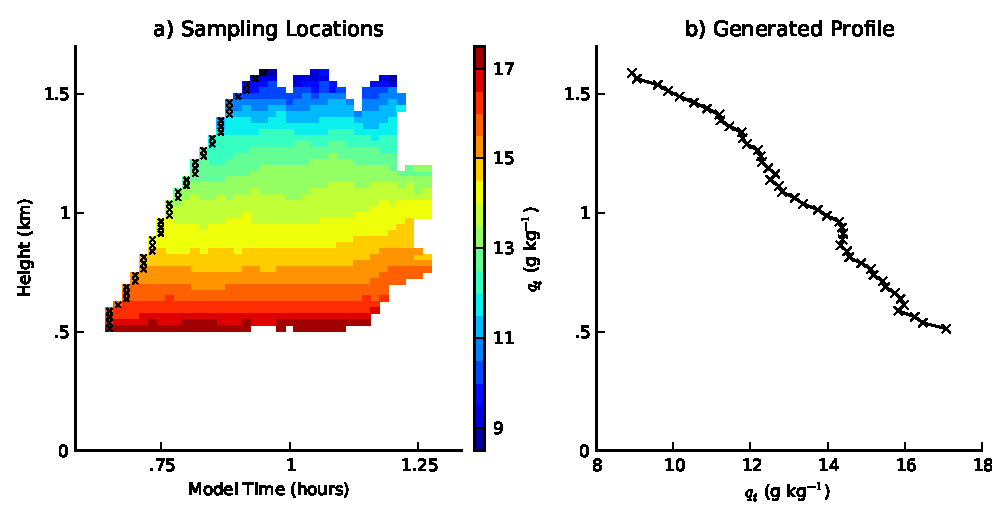
\includegraphics[width=\textwidth]{./figures/cloud_environment_schematic}
\end{center}
\caption{Schematic of encountered cloud environment calculation.}
\label{fig:cloud_environment_schematic}
\end{figure*}

%f
\begin{figure*}[t]
\vspace*{2mm}
\begin{center}
\includegraphics[width=\textwidth]{./figures/placeholder}
\end{center}
\caption{Histograms of encountered cloud environment.}
\label{fig:cloud_envionment_histograms}
\end{figure*}

%f
\begin{figure*}[t]
\vspace*{2mm}
\begin{center}
\includegraphics[width=\textwidth]{./figures/placeholder}
\end{center}
\caption{Schematic of cloud base correlation calculation.}
\label{fig:cloud_base_schematic}
\end{figure*}

%f
\begin{figure*}[t]
\vspace*{2mm}
\begin{center}
\includegraphics[width=\textwidth]{./figures/placeholder}
\end{center}
\caption{Correlation profiles between cloud base and various cloud heights.}
\label{fig:cloud_envionment_histograms}
\end{figure*}


%% TABLES %%%%%%%%%%%%%%%%%%%%%%%%%%%%%%%%%%%%%%%%%%%%%%%%%%%%%%%%%%%%%%%%%%%%


%% ONE-COLUMN TABLE

%t
\begin{table}[t]
\caption{Statistics of tracked clouds}
\vskip4mm
\centering
\begin{tabular}{llcr}
\tophline
&&BOMEX\\
\middlehline
Total Clouds&&1183\\
Starts\\
&Broken&59\\
&Split&339\\
&New&785\\
Ends\\
&Broken&39\\
&Merge&51\\
&Decay&1093\\

\bottomhline
\end{tabular}
\end{table}

%t
%\begin{table}[t]
%\caption{t-test Results}
%\vskip4mm
%\centering
%\begin{tabular}{lcccc}
%\tophline
%&Variable&t-test value&Significance&Direction\\
%\middlehline
%environment&&&\\
%& $q_t$ & -1.33 & 81\% & n/a\\
%& $q_n$ & 0.02 & 2\% & n/a\\
%& tracer & 0.72 & 53\% & n/a\\
%& $\theta_l$ & 2.53 & 98\% & $\downarrow$\\
%& $\theta_v$ & 2.77 & 99.4\% & $\downarrow$\\
%& $w$ & -4.99 & 99.9999\% & $\uparrow$\\
%core&&&\\
%& $q_t$ & 1.57 & 88\% & n/a \\
%& $q_n$ & -0.04 &  3\% & n/a \\
%& $\theta_l$ & -2.10 & 96\% & $\uparrow$ \\
%& $\theta_v$ & -3.55 & 99.96\% & $\uparrow$ \\
% $w$ & -4.21 & 99.997\% & $\uparrow$ \\
%& $\chi_c$ & -5.14 & 99.99995\% & $\uparrow$ \\
%& $a$ & -7.10 & 99.999999992\% & $\uparrow$ \\

%\bottomhline
%\end{tabular}
%\end{table}

%% TWO-COLUMN TABLE

t
\begin{table*}[t]
\caption{t-test results}
\vskip4mm
\centering
\begin{tabular}{lccccccc}
\tophline
&&550-650 m&&650-750 m&&750-850 m& \\
&Variable&t-test value&Significance&t-test value&Significance&t-test value&Significance\\

\middlehline

environment &&       &      &       &      &       & \\
& $q_t$      & -2.12 & 96\% &  0.96 & 66\% &  2.42 & 98\% \\
& $q_n$      &  0.57 & 43\% & -0.17 & 13\% &  1.33 & 81\% \\
& tracer     & -0.81 & 58\% & -0.35 & 27\% &  0.22 & 17\% \\ 
& $\theta_l$ &  1.49 & 86\% & -1.87 & 93\% & -2.80 & 99.4\% \\
& $\theta_v$ &  0.45 & 34\% & -2.12 & 96\% & -2.45 & 98\% \\
& $w$        &  6.45 & 99.999997\% &  3.57 & 99.96\% &  2.03 & 95\% \\
core        &&       &          &       &      &       & \\
& $q_t$      & -2.72 & 99.3\%   & -0.50 & 38\% & -1.25 & 78\% \\
& $q_n$      & -2.76 & 99.4\%   &  0.08 & 6\%  & -0.82 & 58\% \\
& $\theta_l$ &  2.94 & 99.6\%   &  1.15 & 74\% &  1.68 & 90\% \\
& $\theta_v$ & -0.25 & 20\%     &  2.16 & 96\% &  1.28 & 79\% \\
& $w$        &  2.54 & 98\%     &  3.37 & 99.91\% &  1.78 & 92\% \\
& $\chi_c$   &  0.93 & 64\%     &  4.19 & 99.996\% &  0.69 & 51\% \\
& $a$        &  4.31 & 99.997\% &  5.94 & 99.9999991\% &  6.00 & 99.9999992\% \\

\bottomhline
\end{tabular}
\end{table*}


%% The different columns must be seperated with a & command and should
%% end with \\ to identify the column brake.

%%%%%%%%%%%%%%%%%%%%%%%%%%%%%%%%%%%%%%%%%%%%%%%%%%%%%%%%%%%%%%%%%%%%%%%%%%%%%%


%% If figures and tables must be numbered 1a, 1b, etc. the following command
%% should be inserted before the begin{} command.

%\addtocounter{figure}{-1}\renewcommand{\thefigure}{\arabic{figure}a}


\end{document}
